\section{Waffle}
\label{sec:3-instr}

% How does the new features solve the problem?
% ! Change Instruction to Machine Instruction

% TODO: change it more if you can
The key observation for the methodology used in Waffle is that the static analysis and instrumentations collect the required features for evolutionary search techniques in finding inputs that demonstrate worst-case complexity of a test application in a domain-independent way. However, to enable Waffle to efficiently find such inputs, we need to carefully design effective guidance mechanisms to drive Waffle's input generation process. We redesign the evolutionary algorithm of AFL with customized guidance mechanisms that are tailored for finding inputs causing worst-case behavior.

% TODO: Check this out
Figure \ref{fig:waffle-phases} specifies the modules of AFL, in which we made major modifications for intruducing Waffle. The shared memory is designed to be capable of storing the \textit{resource complexity} of an execution. After the memory instantiation, Waffle investigates the source code (of instructions) and inserts instructions for saving performance of a run. In the fuzzing phase, Waffle collects the code coverage and resource usage of the runtime, and utilizes this information for selecting and shrinking the first entry of the queue.

\begin{figure}[!b]
  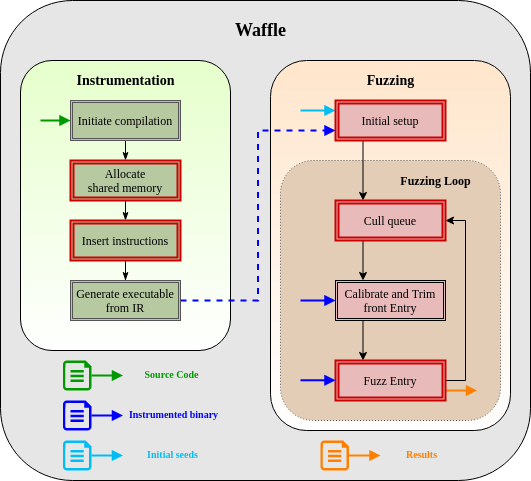
\includegraphics[width=0.8\textwidth]{Chapter3/waffle-proc.png}
  \centering
  \caption{Fuzzing phases of Waffle. The red rectangles specify the changed components.}
  \label{fig:waffle-phases}
\end{figure}

% Explain the modified features from AFL to Waffle
% AFL has become a Waffle :D

% TODO: Rephrase and update this

Next, we will discuss the instrumentation and fuzzing phases of Waffle in more details. To understand the effectiveness of our approach, we first introduce resource complexity of a program and explain how Waffle pivots on this feature for guiding the input generation. After that, the instrumentation phase is extended for discussion, which results in generating an instrumentated binary. The binary file is then passed to the fuzzer, and the evaluation of the inputs takes effect during the fuzzing procedure.

\subsection{Resource complexity of execution}

We define the \textbf{overall resource complexity} (shortened to ORC) of an application as \textit{the amount of resources required to execute a program}. To evaluate the ORC of a program in a concrete execution, each instruction which uses the \textit{engaging resources} should be monitored. For instance, an instruction such as \texttt{memcpy} takes CPU usage for its execution, and may access the program's available memory. A user may track both the CPU and memory usages, and Waffle aggregates the specified resource complexities of the executed instructions to conclude the ORC.

% How does waffle use the complexity

Waffle \textit{estimates} the ORC of each run to guide the input generation process. This estimation is based on a custom set of \textbf{Engaging Instructions} (EI) which represents the machine instructions that are being involved in ORC calculation. For example, suppose that \texttt{memcpy} is the only selected EI; the resources used by only this instruction are then monitored, and the ORC increases for each execution of \texttt{memcpy}. Later, in the fuzzing phase, Waffle uses the ORCs (of EI) to choose the \textit{favored} entries of queue. In AFL, a favored entry is an input which brings something new, in this case \textit{code coverage}. Waffle uses the same technique for detecting code coverages, and additionally, checks the \textit{elite} ORCs of the entries. 



that keeps track of the \textit{most efficient} ORCs that were produced in execution. Waffle updates the content of elite ORCs after culling the queue entries. 

As mentioned in Chapter \ref{chap:ch2}, \texttt{perf\_score} specifies the number of iterations that an input generates fuzzed inputs in havoc mode. Waffle calculates the AFL's \texttt{perf\_score} of a run, and brings in the Engaging Instructions' ORC (EI-ORC) of the execution. The snippet of code \ref{lst:wfl-calc_score} shows the commands that Waffle is using for updating \texttt{perf\_score}, derived from Listing \ref{lst:calc_score}. The value of EI-ORC is computed during the execution with the inserted instructions for incrementing the corresponding indices of the shared array. If the input under fuzzing shows an EI-ORC more than the average EI-ORC of the tests, Waffle increases the iterations for fuzzing the input. The multipliers are set theoretically and they require to be tuned for better results.

\lstinputlisting[language=C,style=CodeStyle,float=tb,label={lst:wfl-calc_score},caption={The added commands for entailing the ORC in \texttt{perf\_score}}]{Codes/Chapter3/waffle-fuzz/calculate_score.c}

\subsection{Instrumentation}
\label{subsec:inst}

% Modifications in memory management

Waffle starts its instrumentation by specifying the shared memory region. Waffle uses two memory regions for this purpose:

\begin{itemize}
  \item An array of 4 bytes cells for tracking the code coverage and the ORC of each basic block. The code coverage works the same as AFL does and the increaments in cells is an attribute for detecting a new path/behavior. The array's length is the same as the AFL's shared array, and as a result, the Waffle's array requires 4x space (Listing \ref{lst:wafl-rt}). Waffle keeps the basic block's ORCs to discover the basic blocks that can contribute more increments in the \texttt{total\_ORC}.
  
  \lstinputlisting[language=C,style=CodeStyle,float=tb,label={lst:wafl-rt},caption={LLVM instrumentation initialization - \texttt{\_\_wafl\_area\_ptr} is the region that is allocated for instruction counters}]{Codes/Chapter3/waffle-llvm-rt.o.c}

  \item To decrease the computational overhead in the fuzzing stage, Waffle stores the summation of all ORCs in an 8 byte integer. As shown in the following code \ref{lst:torc-inst}, function \texttt{addORC} is responsible for adding the value of an ORC to the \texttt{total\_ORC}. The functions \texttt{traceBegin} and \texttt{traceEnd} are assigned with the attributes of constructors and destructors. The constructor is called as this shared library is loaded, and the destructor is called before the file is unloaded. To finilize the storage of \texttt{total\_ORC}, the value is stored in the shared memory when the destructor is being called. 
  
  \lstinputlisting[language=C,style=CodeStyle,label={lst:torc-inst},caption={sys\_data in instrumentation}]{Codes/Chapter3/waffle-fuzz/sys_data_inst.c}
\end{itemize}

% \subsubsection{Visitors}

Waffle uses \textit{LLVM's instruction visitor functions} \cite{inst_visitor} to investigate and count engaging features in the machine code. LLVM provides functions for \texttt{getting} and \texttt{setting} the instructions in a range of address in the code section of the program. This API is applied on the IR of the program and Waffle uses it in the Module Pass of the compilation. Listing \ref{lst:visitors} shows an example of how Waffle implements the counters for instructions; the member function \texttt{visitInstruction(Instruction \&I)} checks if the instruction is of \textbf{any} type, and as a result, an instance of the class \texttt{CountAllVisitor} can contain the occcurences of (any) instructions in a range of instruction pointers.

\lstinputlisting[language=C++,style=CodeStyle,label={lst:visitors},caption={Visitors example}]{Codes/Chapter2/visitor.cpp}

% TODO: Probably explain another example for the counters, like the one checking the memory activities. 
% * Future work: Using different visitor classes? 

A snippet of the Module Pass is shown in Listing \ref{lst:llvm-pass}. In line 6 the pointer to the shared array is introduced; Lines 10 to 14 includes the previously defined function for sum of ORCs, \texttt{addORC()}. After the initial set up, Waffle digs into the basic blocks and create and instance of the \texttt{CountAllVisitor} struct. By passing the current basic block to the visitor, the visitation of EI is stored in \texttt{CAV}. The linear increment in \texttt{CAV} has a relatively large variance in effectiveness of each basic block in changing the total ORC. For instance, if Waffle chooses to count all instructions in the execution, the basic blocks contributed an average of $18$ instructions for the ORC \footnote{Tested C++ implementations of QuickSort, MergeSort, and DFS}. To reduce the impact of large numbers in ORC, Waffle calculates the logarithm of the each counter: 

\begin{equation}
  \label{eq:log}
  CNT = \log_{2}^{CAV+1} 
\end{equation}

The EI-ORC of a basic block is then prepared for storage in both of the storages. Waffle inserts instructions for loading the according index in the shared memory, adds the reduced estimation of EI-ORC to the loaded value, and stores the result back in the same index. Finally, Waffle adds \texttt{CNT} to the \texttt{total\_ORC} by calling the function \texttt{addORC} (Line 42).

\lstinputlisting[language=C,style=CodeStyle,label={lst:llvm-pass},caption={LLVM-mode instrumentation pass}]{Codes/Chapter3/mini-wafl-llvm-pass.so.cc}

Waffle builds its own compiler using the above definitions in instrumentation stage. By making (compiling) the files in \texttt{llvm-mode} directory, an executable compiler, \texttt{waffle-clang} is generated. This compiler scans the source code of the program, and creates a binary file with the logic of the program, and the intended instrumentation:

\begin{lstlisting}[language=bash,style=CommandStyle,label={lst:wafl-clang}]
  ./waffle-clang target.c -o instr_target.bin
\end{lstlisting}